% !TeX root = ../thesis.tex
\section{Background}
The background section will cover four topics.
First the mathematics employed in this project will be covered. This consists of Thiele's differential equation and the fourth-order Runge-Kutta method for solving differential equations.
This is followed by general information on parallelization and why the GPU is particularly effective at it.
After this the CUDA platform, CUDA C and F\# with Alea.cuBase will be discussed.


\subsection{Thiele's differential equation and the Runge-Kutta Method}
The goal of the computations done in this thesis is to estimate the amount of money (reserve) required to be able to fulfil the obligations of a given insurance plan.
Thiele's differential equation\cite{thiele} called ''the fundament of modern life insurance mathematics''\cite{thiele:quote} is a basic tool for determining conditional expected values in intensity-driven Markov processes.
It can be used to express a variety of life insurance products described by multi-state Markov processes.
The equation is expressed below in equation \ref{eq:thiele}. It consists of the following parts:

\begin{itemize}
\item $V_t$ is the reserve at time $t$
\item $\pi_t$ is the premium paid at time $t$
\item $b_t$ is the benefit paid by the insurer at time $t$
\item $\mu_{x+t}$ is the mortality intensity at time $t$ with a person of age age $x$ at the time of signing the contract
\item $r_t$ is interest-rate at time $t$
\end{itemize}

\begin{equation}\label{eq:thiele}
\frac{d}{dt}V_t = \pi_t - b_t \mu_{x+t} + (r_t + \mu_{x+t}) V_t
\end{equation}

With a differential equation such as this, we need a way to solve it. 
The Runge-Kutta method\cite{runge-kutta} is a method for integrating ordinary differential equations by using a trial step at the midpoint of an interval to cancel out lower-order error terms.
The equation can be seen below in equation \ref{eq:rk4}.

\begin{equation}\begin{aligned}\label{eq:rk4}
&k_1 = h f(x_n, y_n)\\
&k_2 = h f(x_n + \frac{1}{2}h, y_n + \frac{1}{2}k_1)\\
&k_3 = h f(x_n + \frac{1}{2}h, y_n + \frac{1}{2}k_2)\\
&k_4 = h f(x_n + h, y_n + k_3)\\
&y_{n+1} = y_n + \frac{1}{6}k_1 + \frac{1}{3}k_2 + \frac{1}{3}k_3 + \frac{1}{6}k_4 + O(h^5)
\end{aligned}\end{equation}

\subsection{Parallelization and the GPU}
Parallelization is the act of taking one task and splitting it into smaller tasks that run concurrently (''in parallel''). This could for example be an algorithm that initially loops $t$ times, but is then altered to instead utilize $t$ tasks that each execute one iteration's work.
This can be done on multi-core CPU's utilizing constructs such as processes and threads, but it can especially be utilized by GPU's that were designed to run operations in parallel for graphics processing.

This is because unlike the CPU which is specialized for data-caching and flow control, the GPU has more transistors dedicated to data processing as illustrated by figure \ref{cpugpu}.

\begin{figure}[h!]
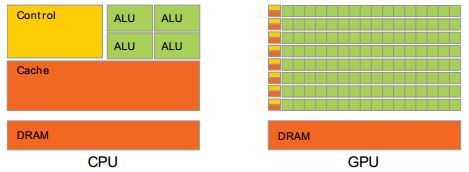
\includegraphics{cpugpu.jpg}
\caption{The GPU devotes more transistors to data processing\cite{cuda_c_programming_guide}\label{cpugpu}}
\end{figure}



Talk about streaming multi-processors. Talk about blocks and threads (+dimensions).
Talk about memory types (shared, global, local, host, etc.)

%http://docs.nvidia.com/cuda/pdf/CUDA_C_Programming_Guide.pdf
%highly parallel, multithreaded, manycore processor with tremendous computational horsepower and very high memory bandwidth
%The reason behind the discrepancy in floating-point capability between the CPU and the GPU is that the GPU is specialized for compute-intensive, highly parallel computation - exactly what graphics rendering is about - and therefore designed such that more transistors are devoted to data processing rather than data caching and flow control
%Talk about GPU vs CPU and parallelization in general

\subsection{CUDA and CUDA C}
CUDA is NVIDIAs parallel computing platform and programming model for harnessing the power of the GPU.
The CUDA platform consists of the CUDA C and C++ languages (referred to as CUDA C from this point), based on C and C++ with some extension and limitations. It also includes parallel computing extensions for other languages such as Fortran and Python. It also includes the CUDA Toolkit which includes a compiler, math libraries and tools for debugging and optimizing performance as well as guides, user manuals, API references and other documentation.

CUDA C is mostly C with added declaration specifiers for methods and variables. The most essential declaration specifier is the \textbf{\_\_global\_\_} specifier which declares a method to be a \textbf{kernel}. Kernels are void-methods that will be executed on the GPU. Code sample \ref{cuda_add} show a simple kernel performing vector addition of the vectors of size $N$.

\begin{lstlisting}[language=C++, caption=CUDA C addition kernel, label=cuda_add]
__global__ void Add(float* a, float* b, float* result){
	//unique id within the kernel
	int i = threadIdx.x + blockIdx.x * blockDim.x;
	// (blockIdx always 0 in this example)
	result[i] = a[i] + b[i];
}

int main(){
	...//Initiate memory on host and device
	Add<<<1, N>>>(a, b, result);
	...//Copy back results, free memory as appropriate
}
\end{lstlisting}

Another thing to note is the launch-parameters of the kernel which specify the amount of blocks and the amount of threads per block. A block can be organized into either one-dimensional, two-dimensional or three-dimensional grids. This is convenient in the case of working with for example matrices, but is not utilized in this thesis and will not be covered in further detail.

CUDA C also has other declaration specifiers. \textbf{\_\_device\_\_} specifies that a method will only be compiled for the GPU (which can be used by kernels), \textbf{\_\_host\_\_} specifies that a method will be available for the CPU. These two specifiers can also be used together for compilation to both platforms.
Variables have the \textbf{\_\_device\_\_} qualifier as well as \textbf{\_\_constant\_\_} to indicate it should be stored in constant memory or \textbf{\_\_shared\_\_} for shared memory.

As it is based on C, dynamic memory must be allocated using malloc and subsequently de-allocated by free.
This operation also has to be done for the device memory using the equivalent cudaMalloc and cudaFree.
The tediousness of this is one of the many benefits from using a more modern language, but at the cost of control that could potentially decrease performance.

\subsection{F\# and Alea.cuBase}
F\#\cite{fsharp} is an open source, cross-platform functional programming language originating from Microsoft that runs on the .NET platform.
Alea.cuBase by QuantAlea\cite{quantalea} is a commercial language integrated compiler for F\# that allows for CUDA development on the .NET platform.
By relying on run-time code-generation it allows for extremely extensible kernels to an extend not easily possible in CUDA C.

It utilizes F\#'s meta-programming support Code Quotation\cite{ms:quotations} for automatic run-time generation of abstract syntax-trees that are then compiled into CUDA's Instruction Set Architecture (ISA) Parallel Thread Execution (PTX) code using Alea.cuBase's compilation API.
Code sample \ref{cubase_add} shows what a simple squaring-kernel could look like in Alea.cuBase F\#. 

\begin{lstlisting}[caption=Alea.cuBase square kernel, label=cubase_add]
let Square = cuda { //use the Alea.cuBase cuda workflow
  let! kernel = <@ fun (a:deviceptr<int>) (result:deviceptr<int>) ->
      let i = blockIdx.x * blockDim.x + threadIdx.x
      result.[i] <- a.[i] * a.[i] @> |> Compiler.DefineKernel
  return Entry(fun program ->
    let worker = program.Worker
    let kernel = program.Apply kernel
    //return host-execution method
    fun (a:int[]) ->
      use a = worker.Malloc(a)
      use result = worker.Malloc(Array.zeroCreate a.Length)
      kernel.Launch (LaunchParam(1, a.Length)) a.Ptr result.Ptr
      result.Gather()) //return result
}

[<EntryPoint>]
let main argv = 
  let a = [| for i in 1 .. 10 -> i |]
  use program = Square |> Compiler.load Worker.Default
  program.Run a |> Array.iter (fun e -> printfn "%d" e)
  0
\end{lstlisting}

The cuda workflow/computation expression (or "monad" for the so inclined) contains the kernel defined with Code Quotations and compiled to an actual kernel and returns a host-side execution method that will handle allocation and deallocation of device-side memory. 
As we are using F\#, the deallocation can be handled automatically by using the use-keyword. 
The program is then loaded to a worker (a CUDA context and background-thread) in the main method compiling the PTX to NVidia internal ISA.
The program is the run using the parameters defined in the run-time method of the cuda workflow (in this case, it just takes an integer array) and the result can be processed on the GPU (in this example, the result is simply printed).